\chapter{\lr{MLOps}}\label{ch:HVS}
 
\section{مقدمه}
 
در حالی که مدل‌های یادگیری ماشین به طور گسترده‌ توسعه یافته‌اند، انتقال آن‌ها از مفهوم آزمایشی به محیط تولید اغلب با شکست مواجه می شود. این فاصله بیشتر به خاطر این است که تاکنون توجه اصلی روی ساخت مدل‌ها بوده است، نه روی تولید محصولات یادگیری ماشین که قابلیت استفاده در محیط تولید را دارند. علاوه بر آن، مدیریت بخش‌ها و زیرساخت‌های پیچیده‌ای که برای یک استقرار موثر ضروری هستند نیز در این امر مغفول مانده اند. برای رفع این مسئله، مفهوم عملیات یادگیری ماشین یا \lr{MLOps} معرفی شده است. \lr{MLOps} بر روی خودکارسازی و عملیاتی کردن فرآیندهای یادگیری ماشین تمرکز دارد تا انتقال پروژه‌های یادگیری ماشین از مفهوم به تولید را تسهیل کند. این رویکرد شامل دیدگاه جامعی از طراحی سیستم، هماهنگی اجزا، تعریف نقش‌ها و مسئولیت‌ها می باشد. هدف کاهش خطا به منظور افزایش قابلیت اطمینان و کارایی سیستم‌های یادگیری ماشین در کاربردهای واقعی می باشد. این فصل به بررسی تعریف، اصول، ابزار و معماری جامعی از یک پلتفرم  \lr{MLOps} پرداخته و در نهایت، محصولات و رقبا این حوزه را بررسی می کنیم.

\section{تعریف مفاهیم اولیه}

\lr{MLOps}
 یا عملیات یادگیری ماشین به مجموعه‌ای از فرایندها، ابزارها و شیوه‌ها جهت مدیریت چرخه توسعه مدل‌های یادگیری ماشین در یک محیط عملیاتی اشاره دارد. همچنین این چرخه شامل همکاری بین دانشمندان داده و مهندسان \lr{DevOps} است به گونه ای که این اطمینان حاصل شود که مدل‌ها به طور مؤثر توسعه، استقرار، پایش و به‌روزرسانی می‌شوند. هدف \lr{MLOps} افزایش سرعت، قابلیت اطمینان و مقیاس پذیری مدل‌های یادگیری ماشین و فرایند توسعه این مدل ها در تولید است؛ درحالی‌که خطرات ناشی از ریسک عدم موفقیت را نیز کاهش می‌دهد. همچنین به‌کارگیری \lr{MLOps} فرایند مدیریت را ساده‌تر کرده، کیفیت را افزایش می‌دهد و استقرار مدل‌های یادگیری عمیق و یادگیری ماشین در محیط‌های تولید با مقیاس بزرگ را خودکار می‌کند. لذا می توان گفت یکی از اهداف \lr{MLOps}، بهبود خودکارسازی و ارتقای کیفیت مدل‌های تولید و درعین‌حال توجه به الزامات تجاری و نظارتی است. 
 
 
 استقرار مدل‌های یادگیری ماشین روی محیط عملیاتی در \lr{MLOps} اهمیت زیادی دارد، زیرا به سازمان‌ها کمک می‌کند تا مطمئن شوند که مدل‌هایشان در طول زمان دقیق، قابل‌اعتماد و کارآمد هستند. به‌طورکلی، \lr{MLOps} با خودکار کردن بسیاری از مراحل مربوط به استقرار و مدیریت مدل‌های یادگیری ماشین، به دانشمندان و مهندسان داده اجازه می‌دهد تا با همکاری یکدیگر به ارائه سریع‌تر و کارآمدتر مدل‌های یادگیری ماشین دست یابند. 
\subsection{اصول}
برای تسهیل در رسیدن به اهداف فوق، تیم‌های \lr{MLOps} از اصول زیر استفاده می کنند:
\begin{enumerate}
	\item 
	خط لوله خودکار \lr{CI/CD} و هماهنگ سازی جریان کار\footnote{\lr{Workflow}}:
	خودکارسازی \lr{CI/CD} شامل مراحل ساخت، آزمایش، تحویل و استقرار است که به توسعه‌دهندگان نسبت به موفقیت یا شکست مراحل مختلف بازخورد سریعی را ارائه داده و بهره‌وری کلی را افزایش می‌دهد \cite{MLOpsPipeline1}. در همین حال، هماهنگ سازی جریان کاری وظایف یک خط لوله‌ یادگیری ماشین را با استفاده از گراف‌های بدون‌حلقه‌ی جهت‌دار\footnote{\lr{Directed Acyclic Graph (DAG)}} هماهنگ می‌کند، که ترتیب اجرای وظایف را با توجه به روابط و وابستگی‌ها تعیین می‌کند. ترکیب این دو رویکرد می ‌تواند به بهبود عملکرد و کارایی تیم‌های توسعه و داده‌کاوی کمک کند \cite{MLOpsWO1, MLOpsWO2}.
	\item 
	کنترل نسخه مدل‌های یادگیری ماشین، مجموعه‌داده‌ها و کد منبع:
با استفاده از نسخه‌بندی مدل، داده و کدمنبع، می‌توان هر تغییر و اصلاحی را در طول زمان دنبال کرد، که این امر به توسعه‌دهندگان و محققان اجازه می‌دهد تا به راحتی به نسخه‌های قبلی بازگردند و نتایج را بازبینی کنند. این قابلیت برای حفظ یکپارچگی و شفافیت در پروژه‌های نرم‌افزاری و علمی بسیار حیاتی است \cite{MLOpsPipeline1}.
	\item 
	نظارت و آموزش مدوام مدل یادگیری ماشین:
آموزش مداوم\footnote{\lr{Continuous Training (CT)}} در یادگیری ماشین به معنای آموزش دوره‌ای مدل‌های یادگیری ماشین بر اساس داده‌های جدید است. این فرآیند همیشه شامل یک مرحله ارزیابی برای سنجش تغییرات کیفیت مدل است \cite{MLOpsCT1}. نظارت مداوم به معنای ارزیابی دوره‌ای داده‌ها، مدل‌ها (مانند دقت پیش‌بینی)، کد منبع و  منابع زیرساختی است تا خطاها یا تغییرات احتمالی که بر کیفیت محصول تاثیر می‌گذارند، شناسایی شوند. این فرآیند به توسعه‌دهندگان امکان می‌دهد تا به سرعت مشکلات را شناسایی و برطرف کنند و از افت عملکرد مدل جلوگیری کنند. یکی از دلایل لزوم آموزش مداوم، رانش داده یا مدل\footnote{\lr{Data or Model Drift}} است، که به تغییرات تدریجی در داده‌ها یا عملکرد مدل در طول زمان اشاره دارد و می‌تواند باعث کاهش دقت پیش ‌بینی‌ها شود \cite{MLOpsProd1}. این اصل در \lr{MLOps} برای اطمینان از عملکرد بهینه مدل‌ها و واکنش سریع به تغییرات محیطی و داده‌ها ضروری است. این فرآیند بهره‌وری را افزایش می‌دهد و کیفیت کلی سیستم‌های یادگیری ماشین را بهبود می‌بخشد. در نهایت، ترکیب آموزش و نظارت مداوم به توسعه‌دهندگان کمک می‌کند تا مدل‌ها را به‌روز نگه داشته و از تاثیرات منفی رانش داده یا مدل جلوگیری کنند \cite{MLOpsCT2}.
	
	\item 
	 ثبت فراداده\footnote{\lr{Metadata}} یادگیری ماشین:
ثبت فراداده برای هر مرحله در جریان ‌کار یادگیری ماشین شامل ثبت جزئیات هر دوره آموزش مدل، مانند تاریخ و زمان آموزش، مدت زمان، پارامترهای استفاده شده و معیارهای عملکرد مدل می باشد \cite{MLOpsWO2}. علاوه بر این، جزئیات مدل که شامل داده‌ها و کدهای استفاده شده است، باید ثبت شود تا قابلیت پیگیری کامل آزمایشات فراهم گردد. این امر به توسعه‌دهندگان کمک می‌کند تا تغییرات و نتایج را به دقت مستند کرده و در صورت نیاز به نسخه‌های قبلی بازگردند \cite{MLOpsProd2}.
	\item 
	حلقه های بازخورد\footnote{\lr{feedback loops}}:
حلقه‌های بازخورد به توسعه‌دهندگان اجازه می‌دهند تا به‌طور مداوم مدل‌ها را بهبود بخشند، مشکلات را شناسایی و رفع کنند و از افت کیفیت جلوگیری کنند. این رویکرد به تضمین کیفیت و کارایی مدل‌های یادگیری ماشین کمک می‌کند و فرآیند توسعه را به یک چرخه تکراری و قابل بهبود تبدیل می‌کند که به سرعت به تغییرات و نیازهای جدید پاسخ می‌دهد \cite{MLOpsProd2}. به عنوان مثال، یک حلقه بازخورد از مرحله مهندسی مدل آزمایشی به مرحله قبلی مهندسی ویژگی می‌تواند بسیار مفید باشد.
\end{enumerate}

می توان اضافه کرد که یکی از اصول مهم که کمتر جنبه فنی دارد و در روح فرهنگی \lr{DevOps} نیز جایگاه ویژه‌ای دارد، اصل همکاری\footnote{\lr{Collaboration}} است. این اصل بر امکان همکاری مشترک افراد بر روی داده‌ها، مدل‌ها و کدها تاکید دارد. علاوه بر جنبه‌های فنی، اصل همکاری به ایجاد فرهنگ کاری مشارکتی توجه دارد که هدف آن کاهش ایزوله سازی ‌های حوزه‌ای بین نقش‌های مختلف است. چنین رویکردی باعث می‌شود تا افراد با تخصص‌های گوناگون به طور هم‌افزا با یکدیگر کار کنند، دانش خود را به اشتراک بگذارند و از هم بیاموزند. 

\subsection{اجزاء}

پس از شناسایی اصولی که در قسمت قبل صحبت کردیم، اکنون اجزای دقیق یک معماری \lr{MLOps} را توضیح داده و ارتباط هرکدام با اصول گفته شده را بیان می کنیم. ارجاعات داخل پرانتز به اصولی اشاره دارد که اجزای فنی در حال پیاده سازی هستند. ؟؟؟؟؟؟؟؟؟؟؟؟؟؟؟؟؟؟؟؟؟؟؟؟؟؟؟؟؟؟؟؟؟؟؟؟؟؟؟؟؟؟؟

\subsubsection{سازآرایی جریان کاری}
سازآرایی جریان‌کاری\footnote{\lr{Workflow Orchestration}} به عنوان یکی از اجزای حیاتی در مدیریت و خودکارسازی جریان‌های کاری پیچیده در حوزه‌های مختلف از جمله یادگیری ماشین و مهندسی داده، نقش مهمی ایفا می‌کنند. این سیستم‌ها مانند شکل 
~\ref{fig: airflow pipelines}
از گراف‌های بدون حلقه جهت دار برای نمایش ترتیب اجرای وظایف استفاده می کنند. هر مرحله از این جریان‌کاری ممکن است شامل استخراج داده، آموزش مدل یا استنتاج باشد. این سیستم‌ها نه تنها ترتیب اجرای وظایف را مدیریت می‌کنند، بلکه وابستگی‌های متقابل بین وظایف را نیز مورد توجه قرار می‌دهند. هم چنین این ابزارها به کاربران امکان می‌دهند تا جریان های کاری را به صورت خودکار و مقیاس ‌پذیر اجرا کنند. این امر به ویژه در محیط‌های بزرگ با داده های کلان اهمیت دارد \cite{MLOpsWO2}.

ابزارهای متن باز معروف در زمینه یادگیری ماشین \lr{Apache Airflow}\cite{Airflow} و \lr{Kubeflow pipeline} می باشند. از \lr{Apache Airlfow} بیشتر برای استخراج، تبدیل و بارگذاری\footnote{\lr{Extract, Transform, Load (ETL)}}داده های بزرگ استفاده می کنند. \lr{Kubeflow Pipelines} نیز بخشی از پلتفرم \lr{Kubeflow}\cite{Kubeflow} است که برای اجرای جریان‌های کاری یادگیری ماشین بر روی کوبرنتیز طراحی شده است \cite{MLOpsWFCOMP1}. از این ابزار به طور خاص برای توسعه و استقرار مدل‌های یادگیری ماشین در محیط‌های ابری مناسب است که در فصل های بعدی با آن بیشتر آشنا خواهیم شد.	

\begin{figure}[t]
	\centering
	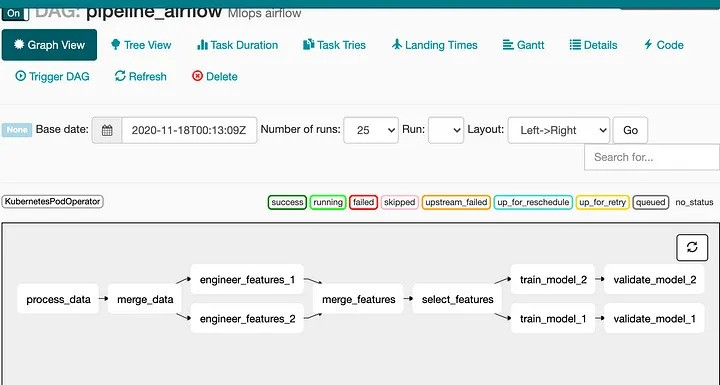
\includegraphics[scale=0.6]{Aairflow-pipeline.jpg}
	\caption{خط لوله در \lr{Apache Airlfow}}
	\label{fig: airflow pipelines}
\end{figure}

\subsubsection{انبار ویژگی}
انباره ویژگی\footnote{\lr{Feature Store}} یک سیستم مدیریت داده است که به منظور ذخیره‌سازی، مدیریت و اشتراک‌گذاری ویژگی‌های مورد استفاده در مدل‌های یادگیری ماشین طراحی شده است. این سیستم (شکل 
~\ref{fig: feature store})
دارای دو بخش اصلی است: پایگاه داده آنلاین و پایگاه داده آفلاین. هر یک از این پایگاه‌های داده نقش خاصی در فرآیند مدیریت و استفاده از ویژگی‌ها ایفا می‌کنند.

\textbf{پایگاه داده آفلاین}
برای ذخیره ‌سازی و مدیریت ویژگی‌هایی استفاده می‌شود که در فرآیندهای آزمایش و تحلیل به کار می‌روند. این پایگاه داده معمولاً با تاخیر نسبتا بیشتری نسبت به پایگاه داده آنلاین استفاده می شود و برای مواردی مناسب است که نیاز به پردازش حجم زیادی از داده‌ها در مدت زمان طولانی ‌تر دارند. ویژگی ‌هایی که در این پایگاه داده ذخیره می‌شوند، اغلب در فرآیندهای آموزش مدل‌های یادگیری ماشین مورد استفاده قرار می‌گیرند.

\textbf{پایگاه داده آنلاین}
برای ارائه ویژگی‌ها به صورت بلادرنگ استفاده می‌شود و تأخیر کمی دارد. این پایگاه داده‌ها برای سیستم‌هایی مناسب هستند که نیاز به پاسخگویی سریع دارند. زمانی که یک مدل یادگیری ماشین نیاز به استفاده از ویژگی‌ها برای انجام پیش‌بینی‌های فوری دارد، داده‌ها از این پایگاه داده آنلاین بازیابی می‌شوند. این نوع پایگاه داده‌ها باید توانایی پشتیبانی از حجم بالای درخواست‌ها را داشته باشند تا بتوانند عملکرد مطلوبی را در شرایط عملیاتی فراهم کنند. ویژگی‌هایی که در این پایگاه داده ذخیره می‌شوند، اغلب در فرآیندهای استنتاج مدل‌های یادگیری ماشین مورد استفاده قرار می‌گیرند.


با استفاده از انباره ویژگی توسعه‌دهندگان می‌توانند ویژگی‌های از پیش پردازش شده را به صورت متمرکز ذخیره کرده و به راحتی در پروژه‌های مختلف به اشتراک بگذارند، که این امر به تسریع فرآیند توسعه مدل‌ها و بهبود دقت پیش بینی ها کمک می‌کند. این سیستم‌ها معمولاً بر روی زیرساخت‌های ابری اجرا می‌شوند تا مقیاس‌پذیری بالا و کارایی مورد نیاز برای پردازش داده های کلان را فراهم کنند \cite{MLOpsCT2}. از ابزار معروف متن باز برای می توان به \lr{Feast}\cite{Feast} اشاره نمود.

\begin{figure}[t]
	\centering
	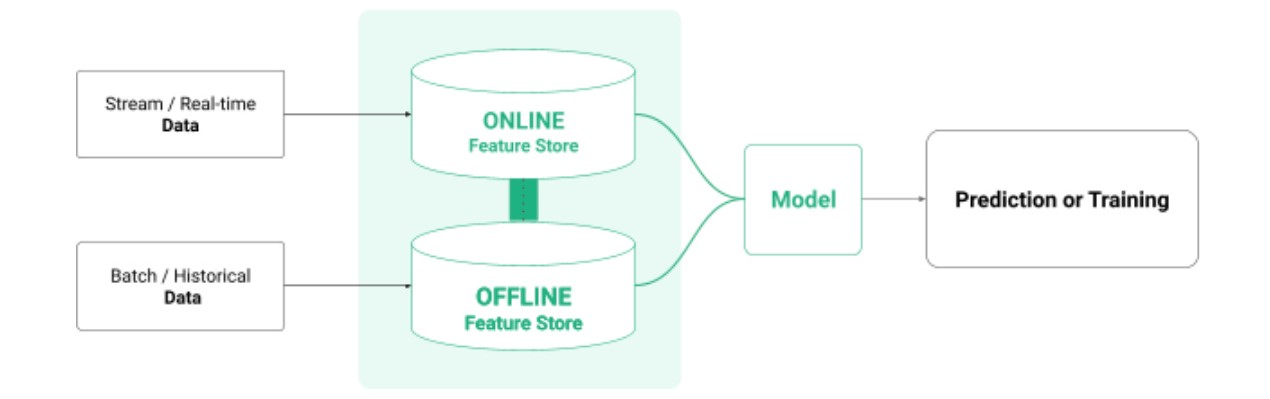
\includegraphics[scale=0.3]{feature-store2.jpg}
	\caption{انباره ویژگی}
	\label{fig: feature store}
\end{figure}

\subsubsection{بانک مدل}
بانک مدل\footnote{\lr{Model Registry}} یکی از ابزارهای بسیار مهم در مدیریت مدل‌های یادگیری ماشین است که به تیم‌ها کمک می‌کنند تا مدل‌های خود را به صورت سازماندهی شده ذخیره، مدیریت و ردیابی کنند. هم چنین اطلاعات مربوط به هر مدل را از جمله نسخه، تاریخ آخرین آموزش، معیارهای ارزیابی و مستندات مربوطه را نگهداری می‌کند. این امر به تیم‌ها کمک می‌کند تا با استفاده از نسخه‌های مختلف مدل‌ها، آزمایش‌های مختلفی انجام دهند و بهترین مدل را انتخاب کنند. هم چنین به هنگام بروز مشکل در مدل های جدید، می توان از مدل های قابل قبول قبلی برای محیط عملیاتی استفاده کرد \cite{MLOpsCloud1}. از ابزار معریف متن باز می توان به \lr{MLflow}\cite{MLflow} اشاره کرد.

\subsubsection{انبار فراداده}
انبار فراداده یادگیری ماشین\footnote{\lr{ML Metadata Store}} برای پیگیری و ذخیره‌سازی اطلاعات مربوط به هر مرحله از جریان کاری یادگیری ماشین استفاده می شوند. فراداده‌ها می‌توانند شامل جزئیاتی نظیر تاریخ و زمان آموزش مدل، مدت زمان هر مرحله از آموزش، پارامترهای استفاده شده، معیارهای عملکرد مدل، و سلسله‌مراتب مدل (مثل داده‌ها و کدهای استفاده شده) باشند. یکی از کاربردهای اصلی انبار فراداده‌ها، مدیریت کارآمد پروژه‌های پیچیده یادگیری ماشین است \cite{MLOpsProd2}. به عنوان مثال، در پروژه‌های بزرگ که شامل آزمایش‌ها و مدل‌های متعددی هستند، پیگیری دقیق و منظم فراداده‌ها می‌تواند به تیم‌ها کمک کند تا نتایج قبلی را به راحتی بازبینی کنند، مشکلات را شناسایی کنند و بهینه‌سازی‌های لازم را انجام دهند. \lr{MLflow}  یک ابزار معروف برای یک سیستم پیشرفته مدیریت فراداده است که همراه با بانک مدل امکان مدیریت یکپارچه مدل‌ها و فراداده‌ها را فراهم می‌کند. 	

\subsubsection{استقرار مدل}
استقرارکردن مدل\footnote{\lr{Model Serving}} به فرآیندی اشاره دارد که در آن مدل‌های یادگیری ماشین آماده برای استفاده، به کار گرفته می‌شوند تا به صورت عملیاتی به پیش‌بینی‌ها و استنتاج‌ها بپردازند. این فرآیند برای تبدیل مدل‌های آموزشی به ابزارهای قابل استفاده در محیط‌های تولیدی ضروری است و می‌تواند به صورت آنلاین برای پیش‌بینی‌های بلادرنگ یا به صورت دسته‌ای\footnote{\lr{Batch}} برای پردازش حجم بالای داده‌ها پیاده‌سازی شود. در محیط‌های عملیاتی، فرآیند استقرار مدل به سه شکل اصلی بلادرنگ، دسته ای و بدون سرور پیاده‌سازی می‌شود \cite{MLOpsCloud1}.

در استنتاج بلادرنگ\footnote{\lr{Real-time Inference}}، مدل‌های یادگیری ماشین به گونه‌ای پیاده‌سازی می‌شوند که بتوانند به سرعت و با کمترین تأخیر ممکن پیش‌بینی‌ها را انجام دهند. این نوع استنتاج برای کاربردهایی نظیر سیستم‌های توصیه‌گر، تحلیل داده‌های حسگرها و برنامه‌های کاربردی که نیاز به پاسخ‌های سریع دارند، مناسب است. به عنوان مثال، در سیستم‌های پیشنهاددهی محتوا مانند نتفلیکس یا آمازون، مدل‌ها باید به صورت بلادرنگ تحلیل کنند و پیشنهادهای شخصی‌سازی شده را ارائه دهند. تکنولوژی‌های مانند \lr{RESTful APIs} و \lr{gRPC} معمولاً برای پیاده‌سازی این نوع سرویس‌دهی استفاده می‌شوند.

استنتاج دسته‌ای\footnote{\lr{Batch Inference}} برای پردازش حجم وسیعی از داده‌ها به کار می‌رود که معمولاً به صورت زمان‌بندی شده انجام می‌شود. این روش برای تحلیل داده‌های کلان و پردازش‌های بزرگ مناسب است. به عنوان مثال، در تجزیه و تحلیل رفتار مشتریان یک فروشگاه آنلاین، داده‌های خریدهای گذشته می‌تواند به صورت دسته‌ای پردازش شود تا الگوهای مختلف شناسایی شود. ابزارهایی مانند \lr{Apache Spark}\cite{Spark} و \lr{Hadoop MapReduce}\lr{Hadoop} معمولاً برای پیاده‌سازی استنتاج دسته‌ای استفاده می‌شوند.

در استنتاج بدون سرور\footnote{\lr{Serverless Inference}}، مدل‌ها به صورت پویا و بر اساس تقاضا اجرا می‌شوند که هزینه و مقیاس‌پذیری را بهینه می‌کند. این نوع استنتاج زمانی مورد استفاده قرار می‌گیرد که نیاز به سرویس‌دهی مقیاس‌پذیر و مقرون‌به‌صرفه باشد. در استنتاج بدون سرور، مدل‌ها فقط زمانی که لازم است اجرا می‌شوند و بنابراین منابع بهینه‌سازی می‌شوند. سرویس‌های ابری مانند \lr{AWS Lambda} و \lr{Google Cloud Functions} معمولاً برای پیاده‌سازی این نوع استنتاج استفاده می‌شوند. از ابزارهای معروف متن باز برای استقرار مدل می توان به \lr{Knative}\cite{Knative} اشاره کرد. 

\subsubsection{نظارت}
نظارت\footnote{\lr{Monitoring}} در یادگیری ماشین یکی از مولفه‌های حیاتی برای تضمین عملکرد بهینه مدل‌ها و زیرساخت‌های مرتبط است. نظارت مداوم بر مدل‌های یادگیری ماشین به دلایلی از  جمله اطمینان از دقت پیش‌بینی‌ها، شناسایی ناهنجاری‌ها و بهبود مداوم عملکرد مدل‌ها ضروری است \cite{MLOpsData}. ابزارهایی مانند \lr{TensorBoard}،\lr{Kubeflow} و \lr{MLflow} نیز نقش مهمی در نظارت بر مدل‌های یادگیری ماشین ایفا می‌کنند. \lr{TensorBoard} به ویژه برای مصورسازی و تحلیل مراحل مختلف آموزش مدل‌ها مفید است. 

نظارت در یادگیری ماشین تنها به مدل‌ها محدود نمی‌شود؛ بلکه زیرساخت‌های مرتبط با یادگیری ماشین نیز نیاز به نظارت دارند. این نظارت شامل نظارت بر فرآیندهای \lr{CI/CD}، هماهنگی سرویس‌ها، خوشه های عملیاتی کوبرنتیز و گره های محاسباتی می‌شود \cite{MLOpsProd2}. یکی از ابزارهای رایج برای نظارت، \lr{Prometheus} است که به همراه \lr{Grafana} برای مصورسازی داده‌ها استفاده می‌شود. علاوه بر این پشته \lr{ELK} (\lr{Elasticsearch}, \lr{Logstash}, \lr{Kibana}) نیز یک مجموعه قدرتمند برای جستجو، تحلیل و مصورسازی لاگ‌های سیستم است که می‌تواند به شناسایی و رفع سریع مشکلات کمک کند. ابزارهای نظارتی به مهندسان اجازه می‌دهند تا هر گونه ناهنجاری در زیرساخت‌ها را به سرعت شناسایی و رفع کنند، که این امر موجب کاهش زمان از کار افتادگی سیستم و افزایش بهره‌وری می‌شود.
 
\subsubsection{زیرساخت آموزش و استقرار مدل}
این زیرساخت شامل منابع محاسباتی اصلی مانند واحد پردازش مرکزی، حافظه واحد پردازش گرافیکی\footnote{\lr{GPU}} است که برای پردازش داده‌ها و اجرای الگوریتم‌های پیچیده می باشد. زیرساخت ها می‌توانند به دو شکل توزیع شده\footnote{\lr{Distributed}} و غیرتوزیع شده پیاده‌سازی شوند. زیرساخت‌های غیرتوزیع‌شده معمولاً شامل ماشین‌های محلی هستند که با وجود سادگی در پیاده‌سازی، محدودیت‌هایی در مقیاس‌پذیری دارند. از سوی دیگر، زیرساخت‌های توزیع‌شده که معمولاً در بستر محاسبات ابری اجرا می‌شوند، امکان توزیع بار کاری بین چندین گره محاسباتی را فراهم می‌کنند و از این طریق مقیاس‌پذیری و کارایی بالاتری ارائه می‌دهند. یکی از ابزار محبوب برای مدیریت و سازآرایی محاسبات توزیع‌شده، کوبرنتیز است که امکان مدیریت کانتینرها و توزیع بار کاری بین گره‌ها را فراهم می‌کند. هم چنین، \lr{Red Hat OpenShift} نیز به عنوان یک پلتفرم دیگر شناخته می‌شود که قابلیت‌های مشابهی ارائه می‌دهد \cite{MLOpsCloud1}.

برای بهینه‌سازی عملکرد مدل‌های یادگیری عمیق، استفاده از واحد پردازش گرافیکی که برای ضرب ماتریسی بهینه‌سازی شده‌اند، استفاده می‌شوند. در دستگاه‌های لبه‌\footnote{\lr{Edge Devices}} به دلیل محدودیت‌های فضا، توان محاسباتی و مصرف انرژی، اجرای مدل‌های یادگیری عمیق پیچیده به چالش‌های خاصی مواجه است. برای غلبه بر این محدودیت‌ها و بهینه‌سازی عملکرد مدل‌ها در این دستگاه‌ها، تکنیک‌های مختلفی مورد استفاده قرار می‌گیرد. یکی از این تکنیک‌ها، استفاده از شبکه‌های عصبی کوانتیزه شده است. در کوانتیزاسیون، وزن‌ها و محاسبات شبکه عصبی از دقت کامل (به عنوان مثال، اعداد با دقت 32 بیت) به اعداد با دقت پایین‌تر (مانند 8 بیت یا حتی کمتر) کاهش می‌یابند. این کاهش دقت باعث کاهش حجم مدل و کاهش نیاز به منابع محاسباتی می‌شود. علاوه بر این، با استفاده از عملیات نقطه شناور کم‌دقت، می‌توان محاسبات را سریع‌تر و با مصرف انرژی کمتری انجام داد. تکنیک دیگر، هرس کردن\footnote{\lr{Pruning}} است که شامل حذف اتصالات غیرضروری و وزن‌های کوچک در شبکه عصبی می‌شود. این فرآیند باعث کاهش تعداد پارامترهای مدل می‌شود، بدون آنکه تاثیر قابل توجهی بر دقت مدل بگذارد. هرس کردن مدل را سبک‌تر و اجرای آن را سریع‌تر می‌کند، که این امر برای دستگاه‌های لبه‌ با منابع محدود بسیار مفید است.


\subsubsection{مخزن کد منبع}
مخزن کد منبع به عنوان یک نقطه مشترک برای نگهداری و مدیریت کدهای مربوط به مدل‌های یادگیری ماشین یک سازمان عمل می‌کند. با استفاده از سیستم‌های مدیریت نسخه مانند گیت، تیم‌ها می‌توانند به راحتی تغییرات کد را پیگیری کرده و در صورت لزوم به نسخه‌های قبلی کد بازگردند. این مخزن همچنین به خودکارسازی فرآیند \lr{CI/CD} کمک می‌کند، به طوری که هرگونه تغییر در کد به طور خودکار خط لوله را فعال کرده و  تغییرات تست، ارزیابی و در محیط‌های مختلف مستقر می‌شوند. می توان از ابزار متن باز برای پیاده سازی آن به \lr{GitLab}\cite{GitLab} و \lr{Gerrit}\cite{Gerrit} اشاره نمود.
\subsubsection{خط لوله \lr{CI/CD}}
همان طور که در گذشته نیز راجع به آن صحبت کردیم، خط لوله \lr{CI/CD} به تیم‌ها اجازه می‌دهند تا کدهای مدل و داده‌ها را به‌صورت مداوم تست، تأیید و استقرار دهند. در این فرآیند، مدل‌ها به طور خودکار بازآموزی و بهبود می‌یابند و در محیط‌های مختلف (توسعه، تست، تولید) به صورت پیوسته به‌روزرسانی می‌شوند. این کار نه تنها باعث افزایش کیفیت و دقت مدل‌ها می‌شود بلکه زمان توسعه و عرضه را نیز به طرز قابل‌توجهی کاهش می‌دهد. در \lr{MLOps} این خط لوله ‌ها در مراحل مختلف از جمله آموزش مدل، ارزیابی، استقرار و نظارت بر عملکرد مدل‌ها و هم چنین داده ها استفاده می‌شوند \cite{MLOpsProd2}. از ابزارهای مناسب برای این کار می توان به \lr{Jenkins}\cite{Jenkins} و \lr{GitLab CI}\cite{GitLab} نام برد. 

\subsection{نقش ها}
در تولید یک پلتفرم \lr{MLOps}، نقش‌های متعددی وجود دارد که همکاری آن‌ها برای طراحی، مدیریت، اتوماسیون و بهره‌برداری از سیستم‌های یادگیری ماشین در محیط تولید بسیار حیاتی است. در ابتدا سهام‌دار کسب‌وکار\footnote{\lr{Business Stakeholder}} وظیفه تعیین اهداف کسب‌وکار و استراتژی بازگشت سرمایه محصول یادگیری ماشین را بر عهده دارد. معمار، معماری سیستم را طراحی کرده و فناوری‌های مناسب را انتخاب می‌کند. دانشمند داده مسئله کسب‌وکار را به مسئله یادگیری ماشین ترجمه کرده و مدل‌ها را مهندسی می‌کند. مهندس داده خط لوله‌های داده و ویژگی را ایجاد و مدیریت می‌کند و داده‌ها را به درستی به سیستم‌های پایگاه داده و انبار ویژگی‌ها تزریق می‌کند. مهندس نرم‌افزار با استفاده از الگوهای طراحی، مسئله یادگیری ماشین را به یک محصول مهندسی‌شده تبدیل می‌کند. مهندس \lr{DevOps} خودکارسازی \lr{CI/CD}، سازآرایی جریان کاری یادگیری ماشین و استقرار مدل در تولید را تضمین می‌کند. در نهایت، مهندس \lr{MLOps} نقش ترکیبی از مهارت‌های چندگانه را دارد و زیرساخت یادگیری ماشین را ایجاد و مدیریت کرده، خط لوله‌های جریان کاری را خودکار می‌کند و مدل‌ها و زیرساخت را در تولید نظارت می‌کند.  این نقش ها که در شکل 
~\ref{fig: mlops roles}
نشان داده شده است، با همکاری و هماهنگی نزدیک می‌توانند \lr{MLOps} را به شکلی مؤثر و کارآمد پیاده‌سازی کنند، که نتیجه آن یک سیستم یادگیری ماشین پایدار و قابل اعتماد در محیط تولید خواهد بود. همکاری میان این نقش‌ها تضمین می‌کند که تمام جنبه‌های مربوط به توسعه، استقرار و نگهداری مدل‌های یادگیری ماشین به درستی مدیریت شود و به اهداف کسب‌وکار دست یابند.
\begin{figure}[t]
	\centering
	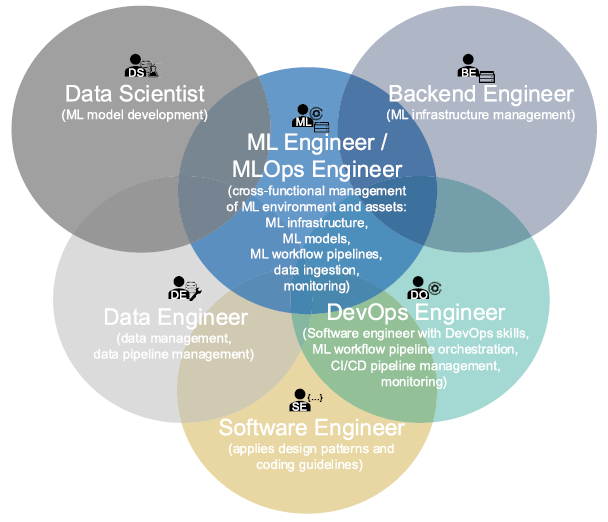
\includegraphics[scale=0.5]{mlops-roles.png}
	\caption{نقش ها و اشتراکات آنها در پارادایم \lr{MLOps}}
	\label{fig: mlops roles}
\end{figure}

\section{معماری کلی}
\begin{figure}[!b]
	\centering
	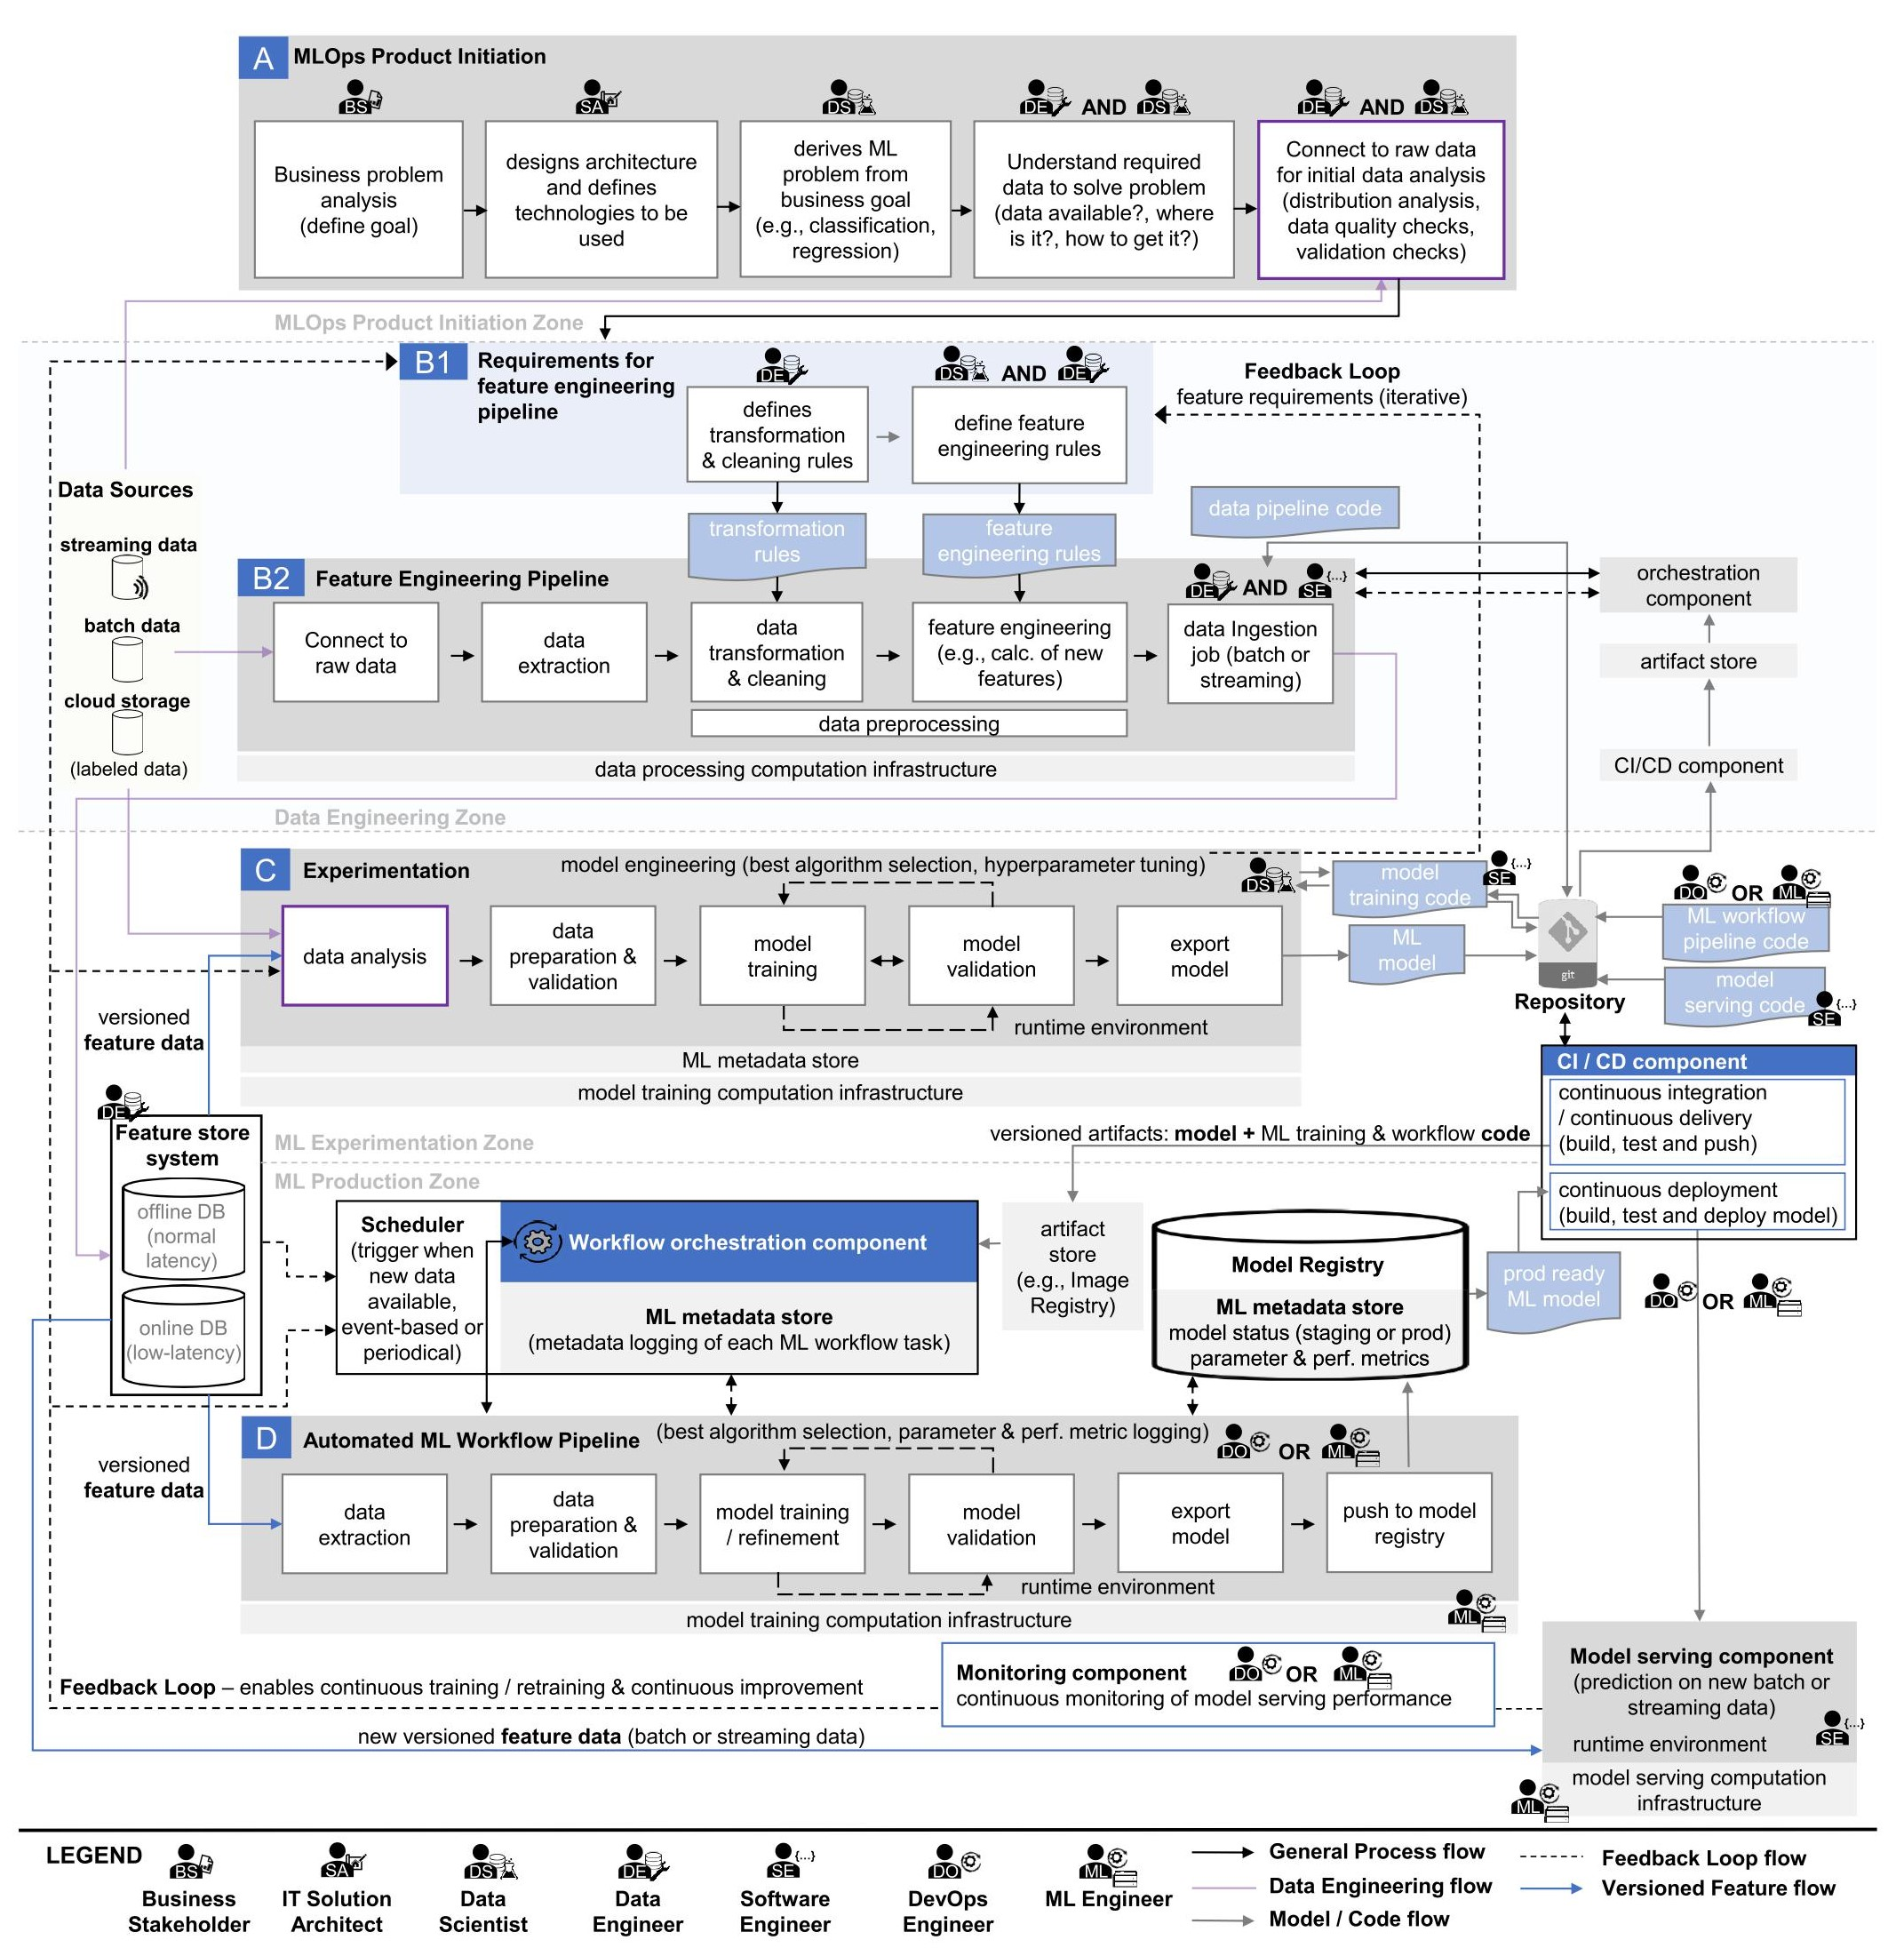
\includegraphics[scale=0.9]{mlops-architecture.jpg}
	\caption{معماری جامع \lr{MLOps}}
	\label{fig: mlops architecture}
\end{figure}
بر اساس اصول، اجزا و نقش‌های بیان شده، یک معماری جامع از یک پلتفرم \lr{MLOps} طراحی شده است. این معماری که در شکل 
~\ref{fig: mlops architecture}
 نشان داده شده جریان‌کارها و ترتیب وظایف در مراحل مختلف را ترسیم می‌کند. این معماری به‌گونه‌ای طراحی شده که کاربران می‌توانند مناسب‌ترین فناوری‌ها و چارچوب‌ها را بر اساس نیازهای خود انتخاب کنند. این انعطاف‌پذیری به کاربران این امکان را می‌دهد که پلتفرم \lr{MLOps} را با استفاده از ترکیبی از ابزارهای متن‌باز، استفاده از سرویس های ابری  یا رویکردهای ترکیبی پیاده‌سازی کنند. نرم‌افزارهای سازمانی و خدمات ابری اغلب از طریق \lr{API}‌ها با ابزارهای متن‌باز یکپارچه می‌شوند و امکان ترکیب بی‌دردسر فناوری‌های مختلف را فراهم می‌کنند. این معماری یک معماری جامع بوده و هر سازمان می تواند برحسب نیاز و هدف خود در حل مسئله یادگیری ماشین، این معماری را شخصی سازی کرده و از پیاده سازی قسمت هایی از آن صرف نظر کند.

\subsubsection{مرحله اولیه}
در فرآیند شروع محصول \lr{MLOps}، اولین مرحله با تحلیل کسب‌وکار آغاز می‌شود. کارشناس مریوط وظیفه دارد تا مشکلاتی را شناسایی کند که با استفاده از یادگیری ماشین قابل حل باشند. پس از شناسایی مشکل، معمار وارد عمل می‌شود. او طراحی معماری کلی سیستم یادگیری ماشین را تعریف کرده و پس از ارزیابی دقیق، تکنولوژی‌های مورد نیاز را انتخاب می‌کند. در مرحله بعدی، دانشمند داده وارد فرآیند می‌شود. دانشمند داده باید از هدف کسب‌وکار، یک مسئله یادگیری ماشین استخراج کند. این مسئله بسته به ماهیت مشکل کسب‌وکار می‌تواند شامل طبقه‌بندی، رگرسیون یا دیگر روش‌های یادگیری ماشین باشد. برای این منظور، دانشمند داده با همکاری مهندس داده باید داده‌های موجود را تجزیه و تحلیل کند تا بهترین رویکرد برای حل مسئله را انتخاب کند. این مرحله نیازمند دانش عمیق از روش‌های مختلف یادگیری ماشین و توانایی تطبیق آن‌ها با نیازهای خاص پروژه است. نکته مهم در این فرآیند، نیاز به داده‌های برچسب‌گذاری‌شده است که برای الگوریتم‌های نظارت‌شده ضروری هستند. در این معماری منابع داده از قبل دارای داده‌های برچسب‌گذاری‌شده بوده‌اند، زیرا فرآیند برچسب‌گذاری در مراحل قبلی انجام شده است.

\subsubsection{خط لوله مهندسی ویژگی}
در فرآیند توسعه مدل‌های یادگیری ماشین، مهندسی ویژگی‌ها\footnote{\lr{Feature Engineering}} به‌عنوان یکی از گام‌های حیاتی شناخته می‌شود که مستلزم تعیین نیازمندی‌های اساسی و پیاده سازی خط لوله مهندسی ویژگی‌ها است. این مرحله شامل تعریف و پیاده‌سازی قواعد تبدیل و پاک‌سازی داده‌ها، و همچنین ایجاد ویژگی‌های جدید و پیشرفته بر اساس ویژگی‌های موجود است. ابتدا نیازمندی‌های مهندسی ویژگی‌ها توسط متخصص داده و مهندس داده تعریف می‌شوند. در این مرحله، قواعد تبدیل داده‌ها\footnote{\lr{Data Transformation}} مانند نرمال‌سازی و تجمیع، و همچنین قواعد پاک‌سازی داده‌ها\footnote{\lr{Data Cleaning}} تعیین می‌شوند تا داده‌ها به فرمت قابل استفاده تبدیل شوند. این قواعد اولیه، به‌صورت تکراری و بر اساس بازخوردهای حاصل از مراحل آزمایشی مهندسی مدل و یا از طریق نظارت بر عملکرد مدل، تنظیم و بهبود می‌یابند.


با تعریف نیازمندی‌های اولیه، مهندس داده و مهندس نرم‌افزار اقدام به ساخت نمونه اولیه خط لوله تولید ویژگی‌ها می‌کنند. این خط لوله باید به صورت مداوم و بر اساس بازخوردهای دریافتی از مراحل مختلف، به‌روزرسانی و بهبود یابد. مراحل کلیدی پیاده‌سازی خط لوله تولید ویژگی‌ها به صورت زیر است:
\begin{itemize}
	\item 
اتصال به داده‌های خام:
اولین مرحله در پیاده‌سازی خط لوله تولید ویژگی‌ها، اتصال به منابع داده خام است. این داده‌ها می‌توانند از منابع مختلفی مانند داده‌های جریانی\footnote{\lr{Streaming Data}}، داده‌های دسته‌ای\footnote{\lr{batch data}} یا داده‌های ذخیره شده در ابر\footnote{\lr{Cloud Storage}}  باشند. داده‌های جریانی به صورت پیوسته و بلادرنگ دریافت می‌شوند، داده‌های دسته‌ای ثابت به صورت دوره‌ای و در حجم بالا جمع‌آوری و پردازش می‌شوند و داده‌های ذخیره شده در ابر از طریق سیستم‌های ابری مقیاس پذیر و انعطاف پذیر ذخیره می‌شوند. اتصال به منابع داده باید به گونه‌ای انجام شود که داده‌ها به راحتی قابل استخراج و پردازش باشند.
	\item 
استخراج داده‌ها:
پس از اتصال به منابع داده، مرحله بعدی استخراج داده‌ها از این منابع است. این مرحله شامل خواندن داده‌ها از پایگاه‌های داده، فایل های \lr{CSV} یا دیگر منابع داده است. 
	\item 
پیش ‌پردازش داده‌ها:
در این مرحله، داده‌های استخراج شده برای تبدیل به فرم قابل استفاده، پیش ‌پردازش می‌شوند. پیش‌ پردازش شامل مراحل مختلفی مانند پاکسازی داده‌ها، مدیریت مقادیر مفقود، حذف نویز، و نرمال‌سازی مقادیر است. هدف اصلی این مرحله، آماده‌سازی داده‌ها به گونه‌ای است که بتوانند به عنوان ورودی‌های مدل یادگیری ماشین استفاده شوند.
	\item 
استخراج ویژگی‌های جدید و پیشرفته: 
یکی از مهم‌ترین مراحل در خط لوله تولید ویژگی‌ها، استخراج ویژگی‌های جدید و پیشرفته است. این ویژگی‌ها بر اساس ویژگی‌های موجود و با استفاده از تکنیک‌های مختلفی مانند ترکیب ویژگی‌ها، اعمال توابع ریاضی، و بهره‌گیری از روش‌های آماری ایجاد می‌شوند. این مرحله به مدل یادگیری ماشین کمک می‌کند تا الگوهای پیچیده‌تری را در داده‌ها شناسایی کند و دقت پیش ‌بینی‌های خود را افزایش دهد.
	\item 
انتقال ویژگی ‌ها به انبار ویژگی‌ها:
در نهایت، داده‌های پردازش شده و ویژگی‌های محاسبه شده به انبار ویژگی‌ها وارد می‌شوند. این انبار می‌تواند شامل پایگاه‌های داده آنلاین یا آفلاین باشد. این بارگذاری باید به گونه‌ای انجام شود که دسترسی سریع و کارآمد به داده‌ها برای مراحل بعدی آموزش مدل فراهم شود.
\end{itemize}

در خط تولید ویژگی‌ها، مهندس نرم افزار به کمک مهندس داده کدهای مورد نیاز برای \lr{CI/CD} و سازآرایی را تعریف می‌کند تا وظایف خط تولید ویژگی‌ها به درستی هماهنگ شوند. این نقش شامل تنظیم منابع زیرساختی برای اطمینان از مقیاس پذیری و عملکرد بهینه خط تولید است. با این تنظیمات، خط تولید ویژگی‌ها می‌تواند به طور مداوم به‌روزرسانی شده و بر اساس بازخوردها بهبود یابد، که این امر بهبود عملکرد مدل‌های یادگیری ماشین را تضمین می‌کند.

برای پیاده‌سازی خطوط تولید ویژگی‌ها، از ابزارها و فناوری‌های مختلفی استفاده می‌شود. برخی از این ابزارها شامل \lr{Apache Spark}، \lr{Apache Kafka} و ابزارهای \lr{ETL} سنتی مانند \lr{Apache Airflow} هستند. \lr{Apache Spark} به دلیل توانایی بالای آن در پردازش موازی و تحلیل داده‌های بزرگ بسیار محبوب است. به عنوان مثال، در یک پروژه پردازش زبان طبیعی\footnote{\lr{Natural Language Processing}} با استفاده از اسپارک، داده‌های متنی بزرگ پردازش و ویژگی‌های متنی جدید محاسبه شدند \cite{MLOpsArchfeature1}. در پروژه دیگری در یک موسسه مالی، داده‌های اعتباری مشتریان با استفاده از اسپارک پردازش و ویژگی‌های مرتبط برای مدل ریسک اعتباری ایجاد شدند \cite{MLOpsArchfeature2}. 
\lr{Apache Kafka} \cite{Kafka} نیز برای بارگذاری داده‌های جریانی بلادرنگ به کار گرفته می‌شود.
هم چنین از \lr{Feast} به همراه پایگاه داده های معروف مانند \lr{PostgreSQL} و \lr{Redis} نیز برای انبار ویژگی ها استفاده می شود.
\subsubsection{بررسی و آزمایش}
مرحله آزمایش مدل در فرآیند یادگیری ماشین یک بخش حیاتی است که بیشتر توسط دانشمند داده به همراه مهندس نرم‌افزار انجام می‌شود. قبل از شروع به کار، مهندس داده به همراه مهندس نرم افزار برای اطمینان از عملکرد درست ابزار و منابع، محیط و سخت افزار را پیکربندی می کنند. حال فرآیند آزمایش مدل شروع می شود:
\begin{itemize}
	\item 
اتصال به انبار ویژگی: 
دانشمند داده به سیستم انبار ویژگی‌ ها متصل می‌شود تا داده‌ها را برای تجزیه و تحلیل دریافت کند. در صورت نیاز، داده خام نیز می‌تواند برای تحلیل‌های اولیه مورد استفاده قرار گیرد. اگر تغییراتی در داده‌ها لازم باشد، این تغییرات به تیم مهندسی داده گزارش می‌شود، که نتیجه آن می تواند منجر به تغییر قواعد تبدیل، پاک سازی داده ها و خط تولید ویژگی ها شود.
	\item 
آماده‌سازی و اعتبارسنجی داده‌ها: 
داده‌ها از سیستم انبار ویژگی‌ها جمع‌آوری و اعتبارسنجی می‌شوند. این مرحله شامل آماده‌سازی داده‌ها و تقسیم آنها به مجموعه‌های آموزش و تست و ارزیابی است تا مدل‌ها بتوانند به طور موثری آموزش داده شوند.
	\item 
آموزش و اعتبارسنجی مدل: 
در این مرحله، دانشمند داده الگوریتم‌های مختلف و پارامترهای آنها را ارزیابی می‌کند تا بهترین ترکیب را پیدا کند. آموزش مدل با استفاده از داده‌های آموزشی شروع می‌شود و مهندس نرم‌افزار در ایجاد کدهای آموزشی بهینه کمک می‌کند. مدل‌ها با استفاده از پارامترهای مختلف به صورت تعاملی آموزش و اعتبارسنجی می‌شوند. این فرآیند تکراری است و تا زمانی که مدل به عملکرد مطلوبی برسد، ادامه می‌یابد. هدف این مرحله شناسایی بهترین الگوریتم و پارامترهای بهینه است. 
	\item 
	استخراج مدل و ثبت کد: 
	پس از شناسایی و انتخاب بهترین مدل، دانشمند داده مدل نهایی را استخراج کرده و کدهای مربوطه را در مخزن کد منبع قرار می دهد. این کدها شامل تمامی اسکریپت‌ها و مستنداتی است که برای تولید، آموزش و ارزیابی مدل استفاده شده‌اند. در همین زمان، مهندس \lr{DevOps} یا مهندس یادگیری ماشین کدهای مربوط به خط لوله یادگیری ماشین را آماده و در مخزن قرار می دهد. این خط لوله شامل اسکریپت‌ها و تنظیماتی است که برای خودکارسازی فرآیندهای مختلف یادگیری ماشین مانند آموزش، ارزیابی و استقرار مدل مورد نیاز است. با انجام این کار، سیستم \lr{CI/CD} به صورت خودکار تغییرات را تشخیص داده و فرآیند ساخت، آزمون و تحویل مدل را آغاز می‌کند. در مرحله ساخت، مصنوعات مدل\footnote{\lr{Model Artifacts}} و کدهای مرتبط ایجاد می‌شوند. در مرحله آزمون، صحت و عملکرد مدل بررسی می‌شود و در نهایت، در مرحله تحویل مدل نهایی به مخزن مصنوعات ارسال می‌شود تا برای استفاده در محیط عملیاتی آماده باشد.	
\end{itemize}

در مرحله آزمایش، ابزارهای مبتنی بر \lr{Notebook} مانند \lr{Jupyter} \cite{Jupyter} به طور گسترده استفاده می‌شوند. این ابزارها به دانشمندان داده اجازه می‌دهند تا داده‌ها را آماده، مدل‌ها را آموزش، ارزیابی و بهینه‌سازی کنند. همچنین برای پیگیری و مدیریت آزمایش‌ها از ابزارهایی مانند \lr{MLflow} و \lr{TensorBoard} استفاده می‌شود.







